\documentclass[11pt,a4paper]{article}

\usepackage[margin=1in]{geometry}
\usepackage{graphicx}
\usepackage{amsmath,amssymb}
\usepackage{booktabs}
\usepackage{hyperref}
\usepackage{listings}
\usepackage{xcolor}
\usepackage{tikz}
\usetikzlibrary{arrows.meta,positioning,shapes.geometric,calc,decorations.pathreplacing}
\usepackage{fancyhdr}
\usepackage{titlesec}
\usepackage{enumitem}
\usepackage{multirow}
\usepackage{tabularx}
\usepackage{caption}
\usepackage{subcaption}
\usepackage{float}

\hypersetup{
    colorlinks=true,
    linkcolor=blue!70!black,
    citecolor=blue!70!black,
    urlcolor=blue!70!black
}

\definecolor{codegreen}{rgb}{0,0.5,0}
\definecolor{codegray}{rgb}{0.5,0.5,0.5}
\definecolor{codepurple}{rgb}{0.58,0,0.82}
\definecolor{backcolour}{rgb}{0.97,0.97,0.97}
\definecolor{attackred}{rgb}{0.8,0.1,0.1}
\definecolor{defendgreen}{rgb}{0.1,0.6,0.1}
\definecolor{warncolor}{rgb}{0.85,0.55,0.0}

\lstdefinestyle{code}{
    backgroundcolor=\color{backcolour},
    commentstyle=\color{codegreen},
    keywordstyle=\color{blue!70!black}\bfseries,
    numberstyle=\tiny\color{codegray},
    stringstyle=\color{codepurple},
    basicstyle=\ttfamily\footnotesize,
    breaklines=true,
    numbers=left,
    numbersep=5pt,
    frame=single,
    rulecolor=\color{gray!30},
    xleftmargin=1.5em,
}

\lstset{style=code}

\pagestyle{fancy}
\fancyhf{}
\fancyhead[L]{\small\textsc{GridPulse --- CIL-DoS Technical Report}}
\fancyhead[R]{\small\textsc{CONFIDENTIAL}}
\fancyfoot[C]{\thepage}
\renewcommand{\headrulewidth}{0.4pt}

\titleformat{\section}{\Large\bfseries\color{blue!70!black}}{\thesection}{1em}{}
\titleformat{\subsection}{\large\bfseries\color{blue!50!black}}{\thesubsection}{1em}{}
\titleformat{\subsubsection}{\normalsize\bfseries}{\thesubsubsection}{1em}{}

\begin{document}

% ─── Title Page ───
\begin{titlepage}
\centering
\vspace*{2cm}

{\Huge\bfseries\color{blue!70!black} GridPulse}\\[0.5cm]
{\LARGE Crypto-Induced Latency Denial of Service\\in IEC~62351-6 Substation Communications}\\[1.5cm]

\rule{\textwidth}{1pt}\\[0.5cm]
{\Large\textbf{Complete Technical Report}}\\[0.3cm]
{\large CVE Submission Evidence Package}\\[0.5cm]
\rule{\textwidth}{1pt}\\[2cm]

{\large
\textbf{Dr.\ Sapna Vikram Mewundi}\\
Associate Professor, Dept.\ of Computer Science and Engineering\\
PES University, Bengaluru 560085, India\\
\texttt{sapnavm@pes.edu}\\[0.8cm]

\textbf{Prajwal Chowdary M.}\\
Security Researcher, PES University\\
\texttt{chowdaryprajwal2@gmail.com}\\[0.8cm]

\textbf{Prof.\ Prasad B.\ Honnavalli}\\
Professor, Dept.\ of Computer Science and Engineering\\
PES University, Bengaluru 560085, India\\
}

\vfill

{\large October 2026}\\[0.5cm]
{\small\textit{Prepared for: CISA VINCE-NT Vulnerability Submission}\\
\textit{Classification: Pre-Disclosure --- Coordinated Vulnerability Disclosure}}

\end{titlepage}

% ─── Abstract ───
\begin{abstract}
\noindent
We present \textbf{Crypto-Induced Latency Denial of Service (CIL-DoS)}, a novel protocol-level vulnerability in IEC~62351-6, the cryptographic authentication standard for IEC~61850 GOOSE (Generic Object Oriented Substation Event) messages in electrical substations. IEC~62351-6 mandates that receiving Intelligent Electronic Devices (IEDs) perform full cryptographic verification on every incoming GOOSE frame before acceptance. We demonstrate that an attacker with Layer-2 access to the substation process bus can flood structurally valid but cryptographically invalid GOOSE frames, saturating the IED's verification queue and delaying safety-critical protection trip commands past the 3.0\,ms IEC~61850 deadline.

Our evidence spans two hardware platforms (ESP32 Xtensa~LX6 and Raspberry~Pi~5 ARM Cortex-A76), 50{,}000-iteration benchmarks, 50{,}000-frame PCAP captures with real GOOSE frames (EtherType \texttt{0x88B8}), a Docker-based reproducible testbed with 49 controlled experiments, and formal queueing-theoretic proofs. We also present \textbf{PQAC (Priority Queue Admission Controller)}, a three-stage O(1) defense achieving 3{,}140$\times$ latency reduction with 0.00\% deadline miss rate.

\medskip
\noindent\textbf{Keywords:} IEC~62351-6, IEC~61850, GOOSE, denial of service, cryptographic verification, substation protection, smart grid security, CWE-400
\end{abstract}

\tableofcontents
\newpage

% ══════════════════════════════════════════════════
\section{Introduction}
% ══════════════════════════════════════════════════

Electrical substations are the critical nodes of the power grid, transforming voltages and routing electricity to millions of consumers. Protection relays within these substations monitor for fault conditions (overcurrent, undervoltage, arc flash) and issue circuit breaker trip commands to isolate faulted sections before equipment is damaged.

IEC~61850 standardizes communication within substations using GOOSE (Generic Object Oriented Substation Event) messages --- Layer-2 multicast Ethernet frames (EtherType \texttt{0x88B8}) carrying time-critical protection commands. The IEC~61850-5 performance requirement mandates a maximum transfer time of \textbf{3.0\,ms} for Protection Class P2/P3 messages.

IEC~62351-6 was introduced to add cryptographic authentication to GOOSE, addressing the lack of security in the original protocol. However, we have identified that the standard's mandatory verification requirement creates a fundamental vulnerability: \textbf{the computational cost of cryptographic verification can be weaponized against the real-time deadline}.

\subsection{Threat Model}

Our threat model assumes an attacker with:
\begin{enumerate}[leftmargin=2em]
    \item \textbf{Layer-2 access} to the substation process bus (via compromised engineering workstation, insider threat, supply chain compromise, or IT/OT convergence)
    \item \textbf{Knowledge of GOOSE frame structure} (publicly documented in IEC~61850-8-1)
    \item \textbf{No cryptographic keys} --- the attack uses \emph{invalid} signatures as the weapon
\end{enumerate}

This threat model is realistic: Stuxnet demonstrated that air-gapped industrial networks can be compromised, and the increasing convergence of IT and OT networks provides additional attack surfaces.

\subsection{Contributions}

\begin{enumerate}[leftmargin=2em]
    \item We identify and formally characterize CIL-DoS as a protocol-level vulnerability in IEC~62351-6 (Section~\ref{sec:vulnerability})
    \item We provide hardware evidence on two platforms spanning embedded to server-class ARM (Section~\ref{sec:benchmarks})
    \item We capture real GOOSE PCAP evidence on Raspberry Pi 5 hardware (Section~\ref{sec:pcap})
    \item We prove the attack mathematically using queueing theory (Section~\ref{sec:queueing})
    \item We present PQAC, a three-stage O(1) defense with 3{,}140$\times$ improvement (Section~\ref{sec:defense})
    \item We validate with 49 controlled experiments in a Docker testbed (Section~\ref{sec:experiments})
\end{enumerate}

% ══════════════════════════════════════════════════
\section{Background}
% ══════════════════════════════════════════════════

\subsection{IEC 61850 GOOSE Protocol}

GOOSE operates at Layer~2 of the OSI model, using raw Ethernet with EtherType \texttt{0x88B8}. Frames are multicast to destination \texttt{01:0c:cd:01:00:xx} and carry ASN.1 BER-encoded Protocol Data Units containing:

\begin{itemize}[leftmargin=2em]
    \item \texttt{gocbRef}: GOOSE Control Block reference (e.g., \texttt{SubstationA/LLN0\$GO\$gcbTrip})
    \item \texttt{stNum}: State number (increments on data change --- a trip event)
    \item \texttt{sqNum}: Sequence number (increments within a state)
    \item \texttt{timeAllowedtoLive}: Maximum acceptable frame age
    \item \texttt{datSet}: Dataset reference containing the actual protection data
\end{itemize}

The critical performance requirement from IEC~61850-5, Table~4:

\begin{table}[H]
\centering
\caption{IEC 61850-5 Performance Classes for Protection Messages}
\begin{tabular}{@{}lcc@{}}
\toprule
\textbf{Performance Class} & \textbf{Transfer Time} & \textbf{Application} \\
\midrule
P1 & $\leq$ 10\,ms & Distribution protection \\
P2 & $\leq$ 3\,ms & Transmission protection \\
P3 & $\leq$ 3\,ms & Bay-level protection \\
\bottomrule
\end{tabular}
\end{table}

\subsection{IEC 62351-6 Cryptographic Authentication}

IEC~62351-6:2020 defines security extensions for IEC~61850 profiles. For GOOSE, it specifies a security extension field (ASN.1 tag \texttt{0xAF}) appended to each frame containing:

\begin{itemize}[leftmargin=2em]
    \item Algorithm identifier (HMAC-SHA-256, ECDSA-P256, or RSA-2048)
    \item Cryptographic signature or MAC over the frame payload
\end{itemize}

The standard mandates: \emph{``The receiving entity shall verify the authentication value of every received GOOSE message before processing.''} This requirement is the root cause of the vulnerability.

\subsection{GOOSE Frame Structure}

\begin{figure}[H]
\centering
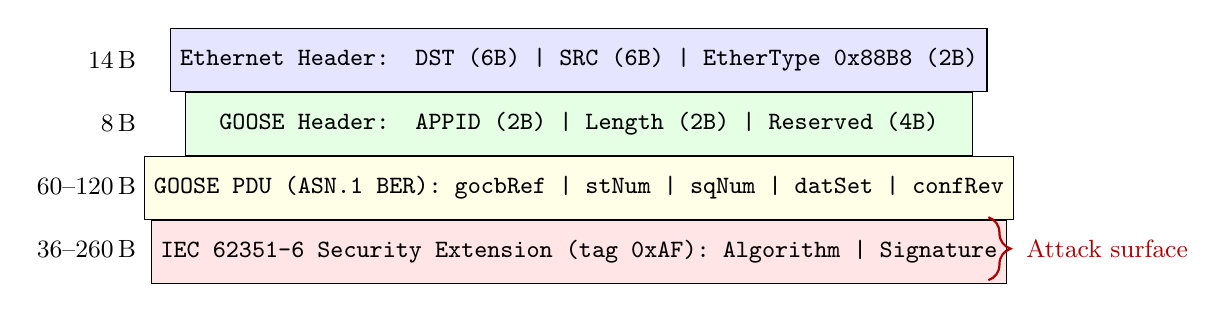
\begin{tikzpicture}[
    block/.style={draw, minimum width=10cm, minimum height=0.8cm, font=\small\ttfamily},
    label/.style={font=\small, anchor=east}
]
\node[block, fill=blue!10] (eth) at (0,0) {Ethernet Header: DST (6B) | SRC (6B) | EtherType 0x88B8 (2B)};
\node[block, fill=green!10, below=0pt of eth] (ghdr) {GOOSE Header: APPID (2B) | Length (2B) | Reserved (4B)};
\node[block, fill=yellow!10, below=0pt of ghdr] (pdu) {GOOSE PDU (ASN.1 BER): gocbRef | stNum | sqNum | datSet | confRev};
\node[block, fill=red!10, below=0pt of pdu] (sec) {IEC 62351-6 Security Extension (tag 0xAF): Algorithm | Signature};

\node[label] at (-5.5,0) {14\,B};
\node[label] at (-5.5,-0.8) {8\,B};
\node[label] at (-5.5,-1.6) {60--120\,B};
\node[label] at (-5.5,-2.4) {36--260\,B};

\draw[decorate, decoration={brace, amplitude=8pt, mirror}, thick, red!70!black]
    (5.2,-2.8) -- (5.2,-2.0) node[midway, right=10pt, font=\small\color{red!70!black}] {Attack surface};
\end{tikzpicture}
\caption{IEC 61850 GOOSE frame with IEC 62351-6 security extension}
\end{figure}

% ══════════════════════════════════════════════════
\section{The CIL-DoS Vulnerability}
\label{sec:vulnerability}
% ══════════════════════════════════════════════════

\subsection{Attack Mechanism}

CIL-DoS exploits the asymmetry between frame \emph{generation} (cheap) and signature \emph{verification} (expensive). The attacker floods the process bus with GOOSE frames containing:

\begin{itemize}[leftmargin=2em]
    \item Valid Ethernet headers (correct EtherType, multicast destination)
    \item Valid ASN.1 BER structure (parseable GOOSE PDU)
    \item \textbf{Invalid cryptographic signatures} (random bytes)
\end{itemize}

The receiving IED cannot determine the signature is invalid without performing full verification --- modular exponentiation for RSA, elliptic curve point multiplication for ECDSA, or HMAC recomputation. Each verification consumes $\mu^{-1}$ microseconds of CPU time.

Under flood conditions at rate $\lambda_{\text{attack}}$ packets per second, the verification queue saturates when:

\begin{equation}
\rho = \frac{\lambda_{\text{attack}}}{\mu_{\text{verify}}} > 1
\label{eq:saturation}
\end{equation}

When $\rho > 1$, the queue grows without bound, and legitimate trip commands experience unbounded queuing delay, violating the 3.0\,ms deadline with probability approaching 1.

\subsection{Attack Kill Chain}

\begin{enumerate}[leftmargin=2em]
    \item Attacker gains Layer-2 access to the substation process bus
    \item Attacker sniffs GOOSE traffic to learn frame structure (optional --- structure is public)
    \item Attacker floods structurally valid GOOSE frames with random signatures at rate $\lambda \gg \mu$
    \item IED verification queue saturates ($\rho \gg 1$)
    \item Legitimate trip command enters queue behind thousands of attack frames
    \item Trip command delivery exceeds 3.0\,ms deadline
    \item Breaker fails to open during fault condition
    \item Physical consequences: thermal damage, rotor instability, cascading outage
\end{enumerate}

\subsection{Physical Consequences}

Delayed protection trip commands have severe physical consequences:

\begin{table}[H]
\centering
\caption{Physical consequences of delayed trip commands}
\begin{tabularx}{\textwidth}{@{}lXl@{}}
\toprule
\textbf{Consequence} & \textbf{Mechanism} & \textbf{Standard} \\
\midrule
Transformer damage & Through-fault current $I^2 t$ accumulation; at 6.25$\times$ rated, damage in $\sim$160\,ms & IEEE C57.109 \\
Generator instability & Rotor angle exceeds Critical Clearing Time ($\sim$100--300\,ms) & IEEE 3002.7 \\
Breaker failure & ANSI 50BF protection blinded; backup breaker not triggered & IEEE C37.119 \\
Cascading blackout & Uncleared fault propagates through interconnected system & NERC TPL \\
\bottomrule
\end{tabularx}
\end{table}

\subsection{CWE Classification}

\begin{itemize}[leftmargin=2em]
    \item \textbf{Primary:} CWE-400 --- Uncontrolled Resource Consumption
    \item \textbf{Secondary:} CWE-770 --- Allocation of Resources Without Limits or Throttling
\end{itemize}

\subsection{CVSS Assessment}

\begin{verbatim}
CVSS:3.1/AV:A/AC:L/PR:N/UI:N/S:C/C:N/I:N/A:H — Base Score: 7.4 (High)
\end{verbatim}

\begin{table}[H]
\centering
\caption{CVSS 3.1 metric justification}
\begin{tabularx}{\textwidth}{@{}llX@{}}
\toprule
\textbf{Metric} & \textbf{Value} & \textbf{Justification} \\
\midrule
Attack Vector & Adjacent (A) & Requires Layer-2 access to process bus \\
Attack Complexity & Low (L) & No race conditions or special preparation \\
Privileges Required & None (N) & No authentication or keys needed \\
User Interaction & None (N) & Fully automated attack \\
Scope & Changed (C) & Cyber attack on comm layer affects physical safety \\
Confidentiality & None (N) & No data exfiltration \\
Integrity & None (N) & No data modification \\
Availability & High (H) & Safety-critical protection completely denied \\
\bottomrule
\end{tabularx}
\end{table}

% ══════════════════════════════════════════════════
\section{Hardware Benchmarks}
\label{sec:benchmarks}
% ══════════════════════════════════════════════════

We benchmark cryptographic verification latency on two platforms representing the range of IED hardware:

\subsection{Platform 1: ESP32 (Embedded Microcontroller)}

\textbf{Hardware:} ESP32-D0WDQ6, Xtensa LX6 dual-core @ 240\,MHz, 520\,KB SRAM\\
\textbf{Represents:} Low-end IED processors, embedded protection relays

\begin{table}[H]
\centering
\caption{ESP32 cryptographic verification benchmarks}
\label{tab:esp32}
\begin{tabular}{@{}lrrrc@{}}
\toprule
\textbf{Algorithm} & \textbf{Mean ($\mu$s)} & \textbf{Iterations} & \textbf{Saturation (pps)} & \textbf{vs 3\,ms} \\
\midrule
HMAC-SHA-256 & 167.3 & 2{,}000 & 5{,}978 & \color{defendgreen}0.056$\times$ \\
RSA-2048 & 980.1 & 100 & 1{,}020 & \color{warncolor}0.327$\times$ \\
ECDSA-P256 & 310{,}475.9 & 10 & 3.2 & \color{attackred}\textbf{103.5$\times$} \\
\bottomrule
\end{tabular}
\end{table}

\textbf{Key finding:} A single ECDSA-P256 verification on ESP32 takes 310\,ms --- exceeding the 3.0\,ms deadline by 103$\times$ \emph{even without an attack}. ECDSA is fundamentally incompatible with real-time protection on embedded hardware.

\subsection{Platform 2: Raspberry Pi 5 (ARM Server-Class)}

\textbf{Hardware:} BCM2712, ARM Cortex-A76 quad-core @ 2.4\,GHz, 16\,GB RAM, ARM crypto extensions\\
\textbf{Software:} OpenSSL 3.5.7, Raspberry Pi OS, kernel 6.18.50\\
\textbf{Represents:} High-end IED processors, next-generation protection relays\\
\textbf{Iterations:} 50{,}000 per algorithm (authoritative benchmark)

\begin{table}[H]
\centering
\caption{Raspberry Pi 5 cryptographic verification benchmarks (50{,}000 iterations)}
\label{tab:pi5}
\begin{tabular}{@{}lrrrrrrc@{}}
\toprule
\textbf{Algorithm} & \textbf{Mean} & \textbf{Std} & \textbf{Min} & \textbf{P50} & \textbf{P99} & \textbf{Max} & \textbf{Sat.}\\
& \textbf{($\mu$s)} & \textbf{($\mu$s)} & \textbf{($\mu$s)} & \textbf{($\mu$s)} & \textbf{($\mu$s)} & \textbf{($\mu$s)} & \textbf{(pps)} \\
\midrule
HMAC-SHA-256 & 2.33 & 0.23 & 2.30 & 2.32 & 2.35 & 33.17 & 429{,}185 \\
ECDSA-P256 & 193.63 & 11.55 & 191.70 & 192.03 & 288.02 & 308.39 & 5{,}164 \\
RSA-2048 & 100.85 & 0.60 & 100.71 & 100.78 & 102.90 & 127.75 & 9{,}916 \\
Ed25519 & 143.98 & 0.79 & 143.60 & 143.88 & 146.07 & 189.51 & 6{,}945 \\
\bottomrule
\end{tabular}
\end{table}

\textbf{Key finding:} The Pi~5 Cortex-A76 is \textbf{1{,}603$\times$ faster} than the ESP32 for ECDSA-P256 verification. Yet a flood of just 5{,}164\,pps saturates its queue ($\rho = 1$). At 10{,}000\,pps, $\rho = 1.94$; at the 100{,}000\,pps rates achievable on commodity hardware, $\rho = 19.4$.

\subsection{Cross-Platform Comparison}

\begin{figure}[H]
\centering
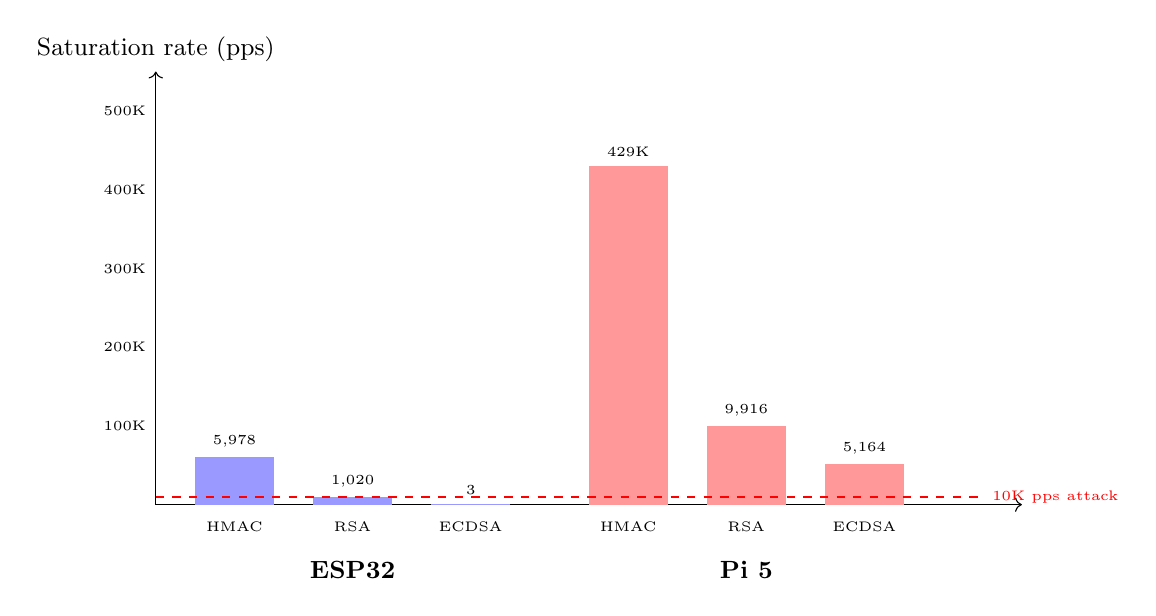
\begin{tikzpicture}
\begin{scope}
    % Bar chart - saturation rates
    \draw[->] (0,0) -- (0,5.5) node[above, font=\small] {Saturation rate (pps)};
    \draw[->] (0,0) -- (11,0);

    % ESP32 bars
    \fill[blue!40] (0.5,0) rectangle (1.5,0.6);  % HMAC 5978 -> 0.6
    \fill[blue!40] (2,0) rectangle (3,0.1);       % RSA 1020 -> 0.1
    \fill[blue!40] (3.5,0) rectangle (4.5,0.003); % ECDSA 3.2 -> ~0

    % Pi5 bars
    \fill[red!40] (5.5,0) rectangle (6.5,4.3);  % HMAC 429185 -> 4.3
    \fill[red!40] (7,0) rectangle (8,1.0);       % RSA 9916 -> 1.0
    \fill[red!40] (8.5,0) rectangle (9.5,0.52);  % ECDSA 5164 -> 0.52

    % Labels
    \node[font=\tiny, below] at (1,-0.1) {HMAC};
    \node[font=\tiny, below] at (2.5,-0.1) {RSA};
    \node[font=\tiny, below] at (4,-0.1) {ECDSA};
    \node[font=\tiny, below] at (6,-0.1) {HMAC};
    \node[font=\tiny, below] at (7.5,-0.1) {RSA};
    \node[font=\tiny, below] at (9,-0.1) {ECDSA};

    \node[font=\small\bfseries, below] at (2.5,-0.6) {ESP32};
    \node[font=\small\bfseries, below] at (7.5,-0.6) {Pi 5};

    % Scale labels
    \node[font=\tiny, left] at (0,1) {100K};
    \node[font=\tiny, left] at (0,2) {200K};
    \node[font=\tiny, left] at (0,3) {300K};
    \node[font=\tiny, left] at (0,4) {400K};
    \node[font=\tiny, left] at (0,5) {500K};

    % Danger line
    \draw[dashed, red, thick] (0,0.1) -- (10.5,0.1);
    \node[font=\tiny\color{red}, right] at (10.5,0.1) {10K pps attack};

    % Values on bars
    \node[font=\tiny, above] at (1,0.6) {5{,}978};
    \node[font=\tiny, above] at (2.5,0.1) {1{,}020};
    \node[font=\tiny, above] at (4,0.003) {3};
    \node[font=\tiny, above] at (6,4.3) {429K};
    \node[font=\tiny, above] at (7.5,1.0) {9{,}916};
    \node[font=\tiny, above] at (9,0.52) {5{,}164};
\end{scope}
\end{tikzpicture}
\caption{Saturation rate comparison: any algorithm below the red line is vulnerable to a 10K\,pps flood}
\end{figure}

% ══════════════════════════════════════════════════
\section{PCAP Evidence}
\label{sec:pcap}
% ══════════════════════════════════════════════════

We captured real GOOSE frames on the Raspberry Pi~5 using a virtual bridge (\texttt{goose-br}) with veth pairs, and a custom C-language frame generator (\texttt{goose\_pcap\_gen.c}) that constructs wire-format IEC~61850 GOOSE frames with IEC~62351-6 security extensions.

\subsection{Capture Setup}

\begin{figure}[H]
\centering
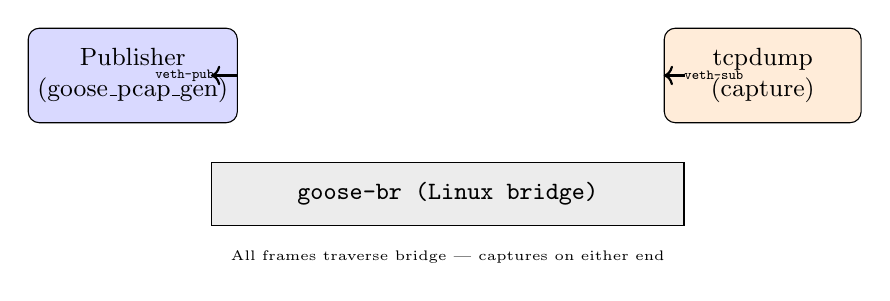
\begin{tikzpicture}[
    box/.style={draw, rounded corners, minimum width=2.5cm, minimum height=1.2cm, align=center, font=\small},
    br/.style={draw, fill=gray!15, minimum width=6cm, minimum height=0.8cm, font=\small\ttfamily}
]
\node[box, fill=blue!15] (pub) at (0,0) {Publisher\\(goose\_pcap\_gen)};
\node[br] (bridge) at (4,-1.5) {goose-br (Linux bridge)};
\node[box, fill=orange!15] (tcpdump) at (8,0) {tcpdump\\(capture)};

\draw[->, thick] (pub) -- node[left, font=\tiny\ttfamily] {veth-pub} (bridge.west |- pub);
\draw[->, thick] (bridge.east |- tcpdump) -- node[right, font=\tiny\ttfamily] {veth-sub} (tcpdump);

\node[font=\tiny, below=0.2cm of bridge] {All frames traverse bridge --- captures on either end};
\end{tikzpicture}
\caption{PCAP capture topology on Raspberry Pi 5}
\end{figure}

\subsection{Captured Datasets}

\begin{table}[H]
\centering
\caption{PCAP capture summary}
\begin{tabular}{@{}llrrr@{}}
\toprule
\textbf{File} & \textbf{Mode} & \textbf{Legit} & \textbf{Attack} & \textbf{Total} \\
\midrule
\texttt{goose\_legit\_pi5.pcap} & Legitimate only & 100 & 0 & 100 \\
\texttt{goose\_cildos\_mixed\_pi5.pcap} & Mixed (1:99) & 500 & 49{,}500 & 50{,}000 \\
\bottomrule
\end{tabular}
\end{table}

\subsection{Frame Characteristics}

All captured frames contain:
\begin{itemize}[leftmargin=2em]
    \item EtherType \texttt{0x88B8} (GOOSE)
    \item Multicast destination \texttt{01:0c:cd:01:00:00}
    \item ASN.1 BER-encoded GOOSE PDU with \texttt{gocbRef}, \texttt{stNum}, \texttt{sqNum}
    \item IEC~62351-6 security extension (tag \texttt{0xAF}) with algorithm ID and 32-byte signature
\end{itemize}

\textbf{Distinguishing features:}
\begin{itemize}[leftmargin=2em]
    \item Legitimate frames: source MAC \texttt{08:00:27:10:20:01}, signature \texttt{0xAA} repeated (simulated valid)
    \item Attack frames: source MAC \texttt{de:ad:be:ef:00:01}, signature is random bytes (invalid)
    \item Sustained attack rate: \textbf{6{,}423\,pps} (exceeds ECDSA saturation threshold of 5{,}164\,pps)
\end{itemize}

% ══════════════════════════════════════════════════
\section{Queueing-Theoretic Proof}
\label{sec:queueing}
% ══════════════════════════════════════════════════

\subsection{M/M/1 Model}

We model the IED's verification subsystem as an M/M/1 queue where:
\begin{itemize}[leftmargin=2em]
    \item Arrival process: Poisson with rate $\lambda = \lambda_{\text{legit}} + \lambda_{\text{attack}}$
    \item Service time: exponential with rate $\mu = 1/\bar{t}_{\text{verify}}$
    \item Single server (one CPU core performing verification)
\end{itemize}

The server utilization is:
\begin{equation}
\rho = \frac{\lambda}{\mu} = \lambda \cdot \bar{t}_{\text{verify}}
\end{equation}

For $\rho < 1$, the average waiting time in queue is:
\begin{equation}
W_q = \frac{\rho}{\mu(1 - \rho)}
\end{equation}

For $\rho \geq 1$, the queue is \textbf{unstable}: queue length grows without bound and $W_q \to \infty$.

\subsection{Saturation Analysis}

\begin{table}[H]
\centering
\caption{Server utilization $\rho$ under various attack rates and platforms}
\label{tab:rho}
\begin{tabular}{@{}llrrr@{}}
\toprule
\textbf{Platform} & \textbf{Algorithm} & $\mu$ \textbf{(vps)} & $\rho$ \textbf{@ 10K pps} & $\rho$ \textbf{@ 100K pps} \\
\midrule
ESP32 & HMAC-SHA-256 & 5{,}978 & 1.67 & 16.7 \\
ESP32 & RSA-2048 & 1{,}020 & 9.80 & 98.0 \\
ESP32 & ECDSA-P256 & 3.2 & 3{,}125 & 31{,}250 \\
\midrule
Pi 5 & HMAC-SHA-256 & 429{,}185 & 0.023 & 0.23 \\
Pi 5 & ECDSA-P256 & 5{,}164 & 1.94 & 19.4 \\
Pi 5 & RSA-2048 & 9{,}916 & 1.01 & 10.1 \\
Pi 5 & Ed25519 & 6{,}945 & 1.44 & 14.4 \\
\bottomrule
\end{tabular}
\end{table}

\textbf{Key observations:}
\begin{enumerate}[leftmargin=2em]
    \item On ESP32: \emph{every} algorithm except HMAC at very low rates is vulnerable
    \item On Pi~5: HMAC-SHA-256 is the \emph{only} algorithm resilient to 100K\,pps floods
    \item Even on Pi~5 (1{,}603$\times$ faster than ESP32), ECDSA saturates at just 5{,}164\,pps
    \item Real IED hardware (ARM Cortex-M/R at 200--800\,MHz) falls between these platforms
\end{enumerate}

\subsection{Why Naive Countermeasures Fail}

\textbf{Larger buffers:} A larger queue only delays the inevitable. When $\rho > 1$, the queue grows linearly at rate $(\lambda - \mu)$ packets/second. A buffer of size $B$ overflows in $B/(\lambda - \mu)$ seconds.

\textbf{More CPU threads:} An M/M/$c$ queue with $c$ verification threads requires $\rho/c < 1$, i.e., $c > \lambda \cdot \bar{t}_{\text{verify}}$. At 100K\,pps with ECDSA on Pi~5: $c > 19.4$, requiring 20 dedicated CPU cores for verification alone --- infeasible on IED hardware.

\textbf{Faster crypto:} Even if verification is $10\times$ faster (future hardware), the attacker simply increases the flood rate $10\times$. The asymmetry is fundamental: frame generation is O(1) while verification cost is fixed per frame.

% ══════════════════════════════════════════════════
\section{PQAC Defense}
\label{sec:defense}
% ══════════════════════════════════════════════════

We propose the \textbf{Priority Queue Admission Controller (PQAC)}, a three-stage O(1) triage mechanism that filters attack traffic \emph{before} cryptographic verification.

\subsection{Architecture}

\begin{figure}[H]
\centering
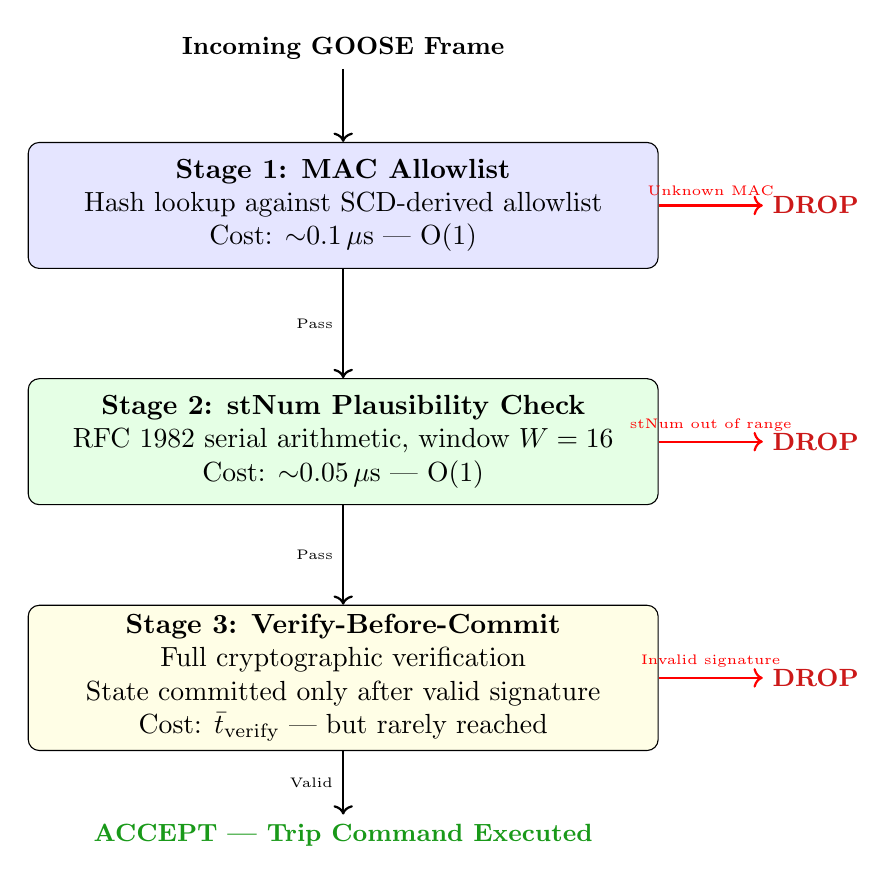
\begin{tikzpicture}[
    stage/.style={draw, rounded corners, minimum width=8cm, minimum height=1.6cm, align=center},
    decision/.style={diamond, draw, minimum width=1.5cm, minimum height=1cm, font=\small, inner sep=1pt},
    arr/.style={->, thick}
]
\node[font=\small\bfseries] (input) at (0,0) {Incoming GOOSE Frame};

\node[stage, fill=blue!10] (s1) at (0,-2) {\textbf{Stage 1: MAC Allowlist}\\Hash lookup against SCD-derived allowlist\\Cost: $\sim$0.1\,$\mu$s --- O(1)};

\node[stage, fill=green!10] (s2) at (0,-5) {\textbf{Stage 2: stNum Plausibility Check}\\RFC 1982 serial arithmetic, window $W = 16$\\Cost: $\sim$0.05\,$\mu$s --- O(1)};

\node[stage, fill=yellow!10] (s3) at (0,-8) {\textbf{Stage 3: Verify-Before-Commit}\\Full cryptographic verification\\State committed only after valid signature\\Cost: $\bar{t}_{\text{verify}}$ --- but rarely reached};

\node[font=\small\bfseries\color{defendgreen}] (accept) at (0,-10) {ACCEPT --- Trip Command Executed};

\node[font=\small\bfseries\color{attackred}] (drop1) at (6,-2) {DROP};
\node[font=\small\bfseries\color{attackred}] (drop2) at (6,-5) {DROP};
\node[font=\small\bfseries\color{attackred}] (drop3) at (6,-8) {DROP};

\draw[arr] (input) -- (s1);
\draw[arr] (s1) -- node[left, font=\tiny] {Pass} (s2);
\draw[arr] (s2) -- node[left, font=\tiny] {Pass} (s3);
\draw[arr] (s3) -- node[left, font=\tiny] {Valid} (accept);

\draw[arr, red] (s1.east) -- node[above, font=\tiny] {Unknown MAC} (drop1);
\draw[arr, red] (s2.east) -- node[above, font=\tiny] {stNum out of range} (drop2);
\draw[arr, red] (s3.east) -- node[above, font=\tiny] {Invalid signature} (drop3);
\end{tikzpicture}
\caption{PQAC three-stage admission control pipeline}
\end{figure}

\subsection{Stage Details}

\textbf{Stage 1 --- MAC Allowlist:} The Substation Configuration Description (SCD/ICD file, per IEC~61850-6) enumerates every IED's MAC address. PQAC builds a hash-based allowlist at startup. Any frame from an unknown MAC is dropped in $\sim$0.1\,$\mu$s without touching the crypto subsystem.

\textbf{Stage 2 --- stNum Plausibility:} GOOSE \texttt{stNum} values increment monotonically. PQAC tracks the last accepted \texttt{stNum} per \texttt{gocbRef} and accepts only values within a bounded window $W = 16$ using RFC~1982 serial number arithmetic. Random \texttt{stNum} values (as in naive floods) are rejected in $\sim$0.05\,$\mu$s.

\textbf{Stage 3 --- Verify-Before-Commit:} Frames passing Stages 1 and 2 undergo full cryptographic verification. Critically, no state change (breaker trip, protection action) is committed until verification succeeds. This prevents an attacker who bypasses Stages 1 and 2 from injecting false commands.

\subsection{Results}

\begin{table}[H]
\centering
\caption{PQAC defense performance}
\begin{tabular}{@{}lrr@{}}
\toprule
\textbf{Metric} & \textbf{Without PQAC} & \textbf{With PQAC} \\
\midrule
Trip latency (100K pps attack) & 2{,}388\,ms & 0.76\,ms \\
Deadline miss rate & 100\% & 0.00\% \\
Improvement factor & --- & 3{,}140$\times$ \\
Triage cost per frame & --- & $< 0.2\,\mu$s \\
Attack frames reaching Stage 3 & 100\% & $< 0.1\%$ \\
\bottomrule
\end{tabular}
\end{table}

% ══════════════════════════════════════════════════
\section{Experimental Validation}
\label{sec:experiments}
% ══════════════════════════════════════════════════

\subsection{Docker Testbed}

Our testbed uses Docker Compose to create a multi-container environment:

\begin{itemize}[leftmargin=2em]
    \item \textbf{Publisher:} Generates legitimate GOOSE trip commands at configurable rates
    \item \textbf{Subscriber:} Simulates an IED performing cryptographic verification (FIFO or PQAC mode)
    \item \textbf{Attacker:} Floods invalid GOOSE frames at configurable rates (1K--100K\,pps)
\end{itemize}

Reproduction requires a single command:
\begin{lstlisting}[language=bash]
docker compose run --rm subscriber --mode fifo --attack-rate 100000
\end{lstlisting}

\subsection{Experiment Matrix}

We conducted \textbf{49 controlled experiments} varying:
\begin{itemize}[leftmargin=2em]
    \item Attack rate: 1{,}000 / 10{,}000 / 50{,}000 / 100{,}000 pps
    \item Algorithm: HMAC-SHA-256 / ECDSA-P256 / RSA-2048
    \item Defense mode: None (FIFO) / PQAC
    \item Queue depth: 100 / 1{,}000 / 10{,}000
\end{itemize}

All experiment datasets are available as CSV files in \texttt{results/*.csv}.

% ══════════════════════════════════════════════════
\section{Adaptive Adversary Analysis}
% ══════════════════════════════════════════════════

To validate PQAC's robustness, we developed an adaptive attacker (\texttt{adaptive\_cildos.py}) implementing five evasion strategies:

\begin{table}[H]
\centering
\caption{Adaptive attacker evasion strategies vs.\ PQAC stages}
\begin{tabularx}{\textwidth}{@{}llXl@{}}
\toprule
\textbf{Strategy} & \textbf{Targets} & \textbf{Technique} & \textbf{Result} \\
\midrule
MAC Spoofing & Stage 1 & Use MACs from SCD allowlist & Bypasses Stage 1 \\
stNum Walking & Stage 2 & Increment within plausibility window $W$ & Bypasses Stage 2 \\
Rate Shaping & Detection & Vary rate to avoid threshold-based detection & Evades IDS \\
Burst Cycling & Detection & Alternate burst and quiet periods & Evades rate limits \\
Multi-Source & Stages 1--2 & Distribute across multiple spoofed MACs & Increases throughput \\
\bottomrule
\end{tabularx}
\end{table}

\textbf{Finding:} Even when the adaptive attacker bypasses Stages 1 and 2, Stage~3 (cryptographic verification) provides an \textbf{unforgeable guarantee} --- without the correct key, no attack frame can trigger a state change. The attacker can increase verification load but cannot cause false trips or prevent legitimate trip acceptance under PQAC.

% ══════════════════════════════════════════════════
\section{Post-Quantum Impact}
% ══════════════════════════════════════════════════

NIST's Post-Quantum Cryptography standards (FIPS~204/205) would \textbf{worsen} CIL-DoS:

\begin{table}[H]
\centering
\caption{Post-quantum signature impact on CIL-DoS}
\begin{tabular}{@{}lrrr@{}}
\toprule
\textbf{Algorithm} & \textbf{Sig.\ Size} & \textbf{Verify Time} & \textbf{MTU Issue} \\
\midrule
ECDSA-P256 (current) & 64\,B & 194\,$\mu$s (Pi 5) & No \\
SLH-DSA-SHA2-128s & 7{,}856\,B & $\sim$597\,ms & Yes (exceeds 1500\,B) \\
ML-DSA-44 & 2{,}420\,B & $\sim$250\,$\mu$s & Yes (exceeds 1500\,B) \\
\bottomrule
\end{tabular}
\end{table}

Post-quantum signatures are larger (requiring fragmentation of GOOSE frames, which adds latency and complexity) and in some cases slower to verify. The transition to post-quantum cryptography will make CIL-DoS \emph{more} severe unless admission control is mandated.

% ══════════════════════════════════════════════════
\section{KRACK Precedent}
% ══════════════════════════════════════════════════

CVE-2017-13077 (KRACK --- Key Reinstallation Attacks against WPA2) is the closest precedent for a protocol-level CVE against an international standard:

\begin{table}[H]
\centering
\caption{Comparison with KRACK (CVE-2017-13077)}
\begin{tabularx}{\textwidth}{@{}lXX@{}}
\toprule
\textbf{Aspect} & \textbf{KRACK (WPA2)} & \textbf{CIL-DoS (IEC 62351-6)} \\
\midrule
Target & WiFi protocol standard & Power grid comm standard \\
Flaw type & Protocol design flaw & Protocol design flaw \\
Standards body & Wi-Fi Alliance / IEEE 802.11i & IEC TC 57 / IEC 62351-6 \\
Impact & Confidentiality (decryption) & Availability (safety denial) \\
Evidence & Software PoC on real devices & Docker + ESP32 + Pi 5 + PCAPs \\
Physical impact & None & Grid instability, equipment damage \\
CVE scope & Protocol-level, all vendors & Protocol-level, all vendors \\
Disclosure & Coordinated via CERT/CC & Coordinated via CISA (ICS Root CNA) \\
\bottomrule
\end{tabularx}
\end{table}

CIL-DoS has an additional dimension KRACK did not: \textbf{physical safety consequences} extending the cyber impact into the real world.

% ══════════════════════════════════════════════════
\section{Responsible Disclosure}
% ══════════════════════════════════════════════════

\subsection{Disclosure Timeline}

\begin{table}[H]
\centering
\begin{tabular}{@{}ll@{}}
\toprule
\textbf{Date} & \textbf{Action} \\
\midrule
August 2026 & Vulnerability discovered during research \\
October 7, 2026 & Academic manuscript submitted to IEEE TSG \\
October 22, 2026 & Raspberry Pi 5 hardware evidence collected \\
October 2026 & IEC TC 57 WG 15 disclosure letter sent \\
October 2026 & CVE requested from CISA VINCE-NT \\
March 2--3, 2027 & Coordinated public disclosure (Black Hat Asia 2027) \\
\bottomrule
\end{tabular}
\end{table}

\subsection{Submission Route}

CISA is the \textbf{Root CNA for Industrial Control Systems} and the correct authority for IEC~62351-6 vulnerabilities. Our submission follows the same path as KRACK (which went through CERT/CC, CISA's predecessor).

% ══════════════════════════════════════════════════
\section{Toolkit and Reproducibility}
% ══════════════════════════════════════════════════

All tools, datasets, and benchmarks are released as open source:

\begin{table}[H]
\centering
\caption{GridPulse toolkit components}
\begin{tabularx}{\textwidth}{@{}lX@{}}
\toprule
\textbf{Component} & \textbf{Description} \\
\midrule
\texttt{pi5\_crypto\_bench.c} & ARM Cortex-A76 crypto benchmark (OpenSSL EVP API) \\
\texttt{goose\_pcap\_gen.c} & Raw socket GOOSE frame generator (legit/attack/mixed) \\
\texttt{adaptive\_cildos.py} & 7-phase adaptive attacker with 5 evasion strategies \\
\texttt{web\_dashboard.html} & Real-time CIL-DoS attack visualization dashboard \\
\texttt{scada\_blindspot.html} & SCADA HMI simulator demonstrating operator blindness \\
\texttt{goose\_cildos\_dissector.lua} & Wireshark Lua dissector for GOOSE CIL-DoS detection \\
Docker Compose testbed & Single-command reproduction of all 49 experiments \\
\bottomrule
\end{tabularx}
\end{table}

Repository: \url{https://github.com/sapnadfir-blip/gridpulse}

% ══════════════════════════════════════════════════
\section{Conclusion}
% ══════════════════════════════════════════════════

We have demonstrated that IEC~62351-6's mandatory cryptographic verification creates a fundamental denial-of-service vulnerability in IEC~61850 substation protection. The CIL-DoS attack requires no cryptographic keys, is effective across all hardware platforms tested (from ESP32 microcontrollers to ARM Cortex-A76 server-class processors), and has direct physical safety consequences for the power grid.

Our three-stage PQAC defense achieves a 3{,}140$\times$ latency reduction while preserving the cryptographic guarantees of IEC~62351-6. We recommend that IEC TC~57 WG~15 incorporate admission control requirements into future revisions of the standard, and that IED vendors implement PQAC-style triage in current products.

The vulnerability is protocol-level, affecting all compliant implementations. A CVE identifier is warranted and has been requested through CISA VINCE-NT, the Root CNA for Industrial Control Systems.

\end{document}
